\documentclass[tikz]{standalone}
\usetikzlibrary{arrows.meta}
\begin{document}
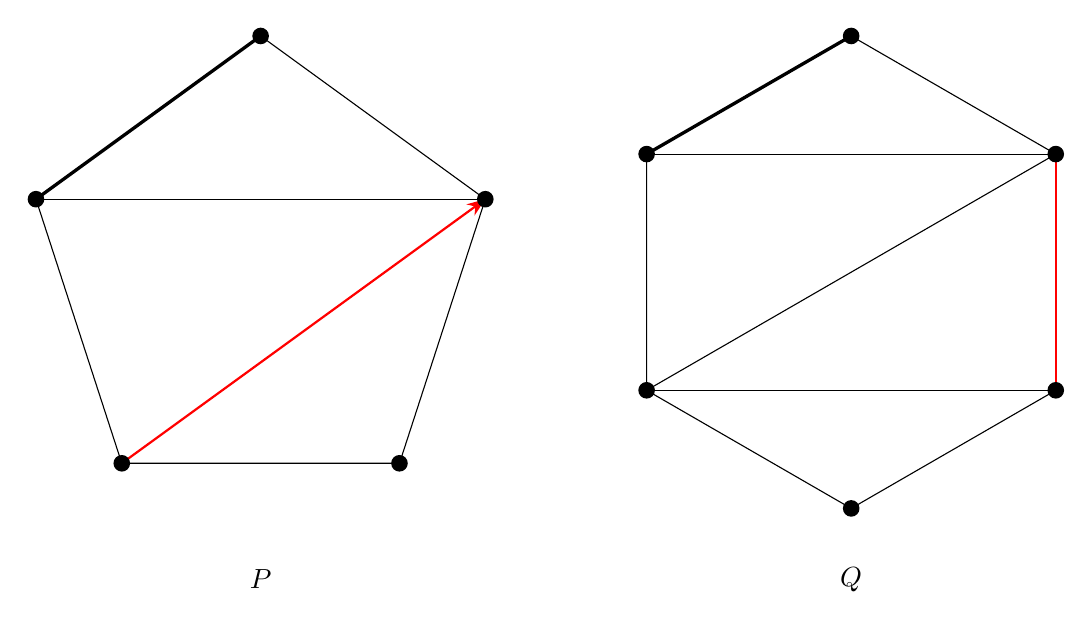
\begin{tikzpicture}[scale=3, every node/.style={circle, inner sep=1pt}]

% Pentagon
\begin{scope}
  \foreach \i [count=\j from 1] in {90,162,234,306,18} {
    \coordinate (P\j) at (\i:1);
  }
  \draw (P1) -- (P2) -- (P3) -- (P4) -- (P5) -- cycle;
  \draw[very thick] (P1) -- (P2);
  \draw (P2) -- (P5);
  \draw[red,thick,->,>=Stealth] (P3) -- (P5);
  \foreach \j in {1,...,5} {
  \fill (P\j) circle (1pt);
}
\node at (0,-1.3) {$P$};
\end{scope}

% Hexagon
\begin{scope}[xshift=2.5cm]
  \foreach \i [count=\j from 1] in {90,150,210,270,330,30} {
    \coordinate (H\j) at (\i:1);
  }
  \draw (H1) -- (H2) -- (H3) -- (H4) -- (H5) -- (H6) -- cycle;
  \draw[very thick] (H1) -- (H2);
  \draw (H2) -- (H6);
  \draw (H3) -- (H6);
  \draw (H3) -- (H5);
  \draw[red,thick] (H5) -- (H6);
  \foreach \j in {1,...,6} {
    \fill (H\j) circle (1pt);
  }
  \node at (0,-1.3) {$Q$};
\end{scope}

\end{tikzpicture}
\end{document}
